\documentclass{article}
\usepackage[backend=biber]{biblatex}
\usepackage[]{hyperref}
\usepackage{graphicx}
\usepackage{booktabs}
\addbibresource{bibliography.bib}
\author{De Trane Giorgio\\s275514}
\title{\textbf{Esercitazioni Strutture\\per Veicoli Spaziali}}

\begin{document}
    \maketitle
    \begin{center}
        \includegraphics[width=0.8\textwidth]{polito_logo.png}
        \linebreak
        \linebreak
        \textit{Anno accademico\\2020-2021}
    \end{center}
    \pagebreak
    \section{Esercitazione 1}
    L'esercitazione é svolta utilizzando uno script in Fortran, messo a disposizione
    in un archivio denominato \textit{MUL2} \autocite*{MUL2} e contenente anche un file di input ad hoc, in formato \textit{.dat},
    oltre a degli utili script di esempio per \textit{gnuplot} \autocite*{gnuplot}, un libre software utilizzato poi per plottare tutti i grafici che seguono.

        \subsection{Esempio}
        Il caso esaminato é quello dell'Esempio 2, i cui dati sono quelli
        forniti di default nel file input.dat .\\
        La configurazione in esame consiste in due camere comunicanti attraverso
        una ventilazione passiva, con un breach sull'ambiente esterno. 
        \begin{center}
            
        
            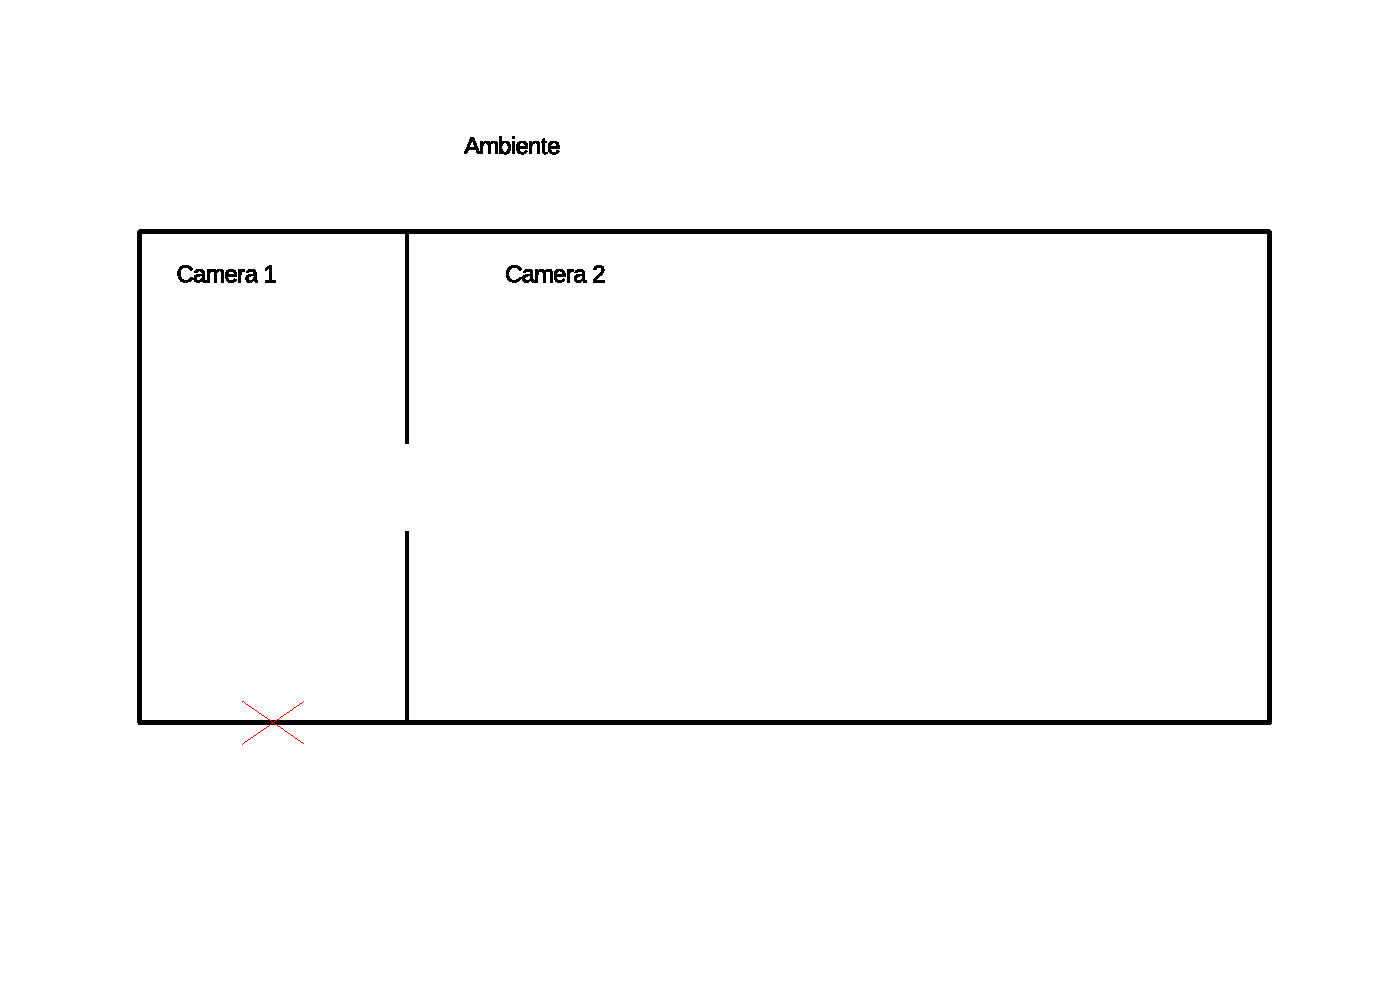
\includegraphics[width=0.9\textwidth]{ES1_Esempio2.eps}
        \end{center}
        \pagebreak
        \printbibliography
\end{document}